% !TEX root = ../thesis.tex
\chapter{Technical Preliminaries}
\label{chapter:technical_preliminaries}
\thispagestyle{empty}

The aim of this chapter is to provide the reader with preliminary notions about the technical knowledge necessary to understand the functioning of the adopted tools, which will be described later in Chapter~\ref{chapter:techniques}.

We will start by introducing \textit{relational databases}, the \textit{data science pipeline} and \textit{data mining techniques}, and then focusing on more specific concepts such as \textit{linear regression} and \textit{functional dependencies}. Finally, an explanation of some needed \textit{evaluation metrics} and \textit{statistical concepts} will follow.

As specified in Chapter~\ref{chapter:socio-ethical_preliminaries}, the complementarity of the preliminaries is one of the key points of this research, and will allow the reader to have two perspectives of a different nature on the same problem.


\section{Relational Databases}
\label{section:relational_databases}
When dealing with computer systems, one of the most basic notions, often inappropriately taken for granted, is the one of `\textbf{data}', definable as:
\begin{quote}\emph{Information, especially facts or numbers, collected to be examined and considered and used to help decision-making, or information in an electronic form that can be stored and used by a computer.} \cite{cambridge2013data}\end{quote}
Therefore, a large amount of data stored in a computer in some organized manner is called a \textbf{database}. To be more precise, a database is ``any collection of data, or information, that is specially organized for rapid search and retrieval by a computer'' \cite{britannica2020database}; while the software that supports the management of these data is called a \textbf{Database Management System (DBMS)}.

The history of databases is deeply interconnected with the history of computer science itself, because the problem of how to store and retrieve information appeared as one of the initial challenges of computer creators. However, in the past few decades the rapid and enormous evolution of computer systems and databases led to the adoption and the development of the so-called `data models'. A \textbf{data model} \cite{abiteboul1995foundations} is an abstract representation of an information system, which defines the data elements and the relationships between data elements. The aim of a data model is to give a clear and intuitive overview on how a system looks like, by providing a standardized description of its components, in such a way as to facilitate the understanding of the system itself and the possible integration with other systems.

Nowadays, the most widespread data model is the \textbf{relational model}, firstly proposed by Codd in \cite{codd1970relational}. The relational model represents a database as a collection of relations, depicted as tables of values. Each row of the table is a collection of related data values, referring to a real-world entity or relationship between entities. Therefore, we can simply define a \textbf{relational database} as a digital database based on the relational model of data.
To make it clearer, the following list provides the main terms used in this context, together with a concise explanation, while Figure~\ref{fig:relational_model} shows them in a trivial example.
\begin{itemize}
\item \textbf{Table}, or \textbf{relation}: modeling of a real-world entity or of a relationship between real-world entities.
\item \textbf{Row}, or \textbf{tuple}: single data record.
\item \textbf{Column}, or \textbf{attribute}: property, or feature, of a relation.
\item \textbf{Cardinality}: total number of tuples of a relation.
\item \textbf{Degree}: total number of attributes of a relation.
\item \textbf{Primary key}: attribute, or combination of attributes, that uniquely identifies a tuple among the others.
\item \textbf{Domain}, or \textbf{data type}: set of values that a specific attribute can assume (for example, integer numbers, or boolean values).
\item \textbf{Database schema}, or simply \textbf{schema}: blueprint of the database that outlines the way its structure organizes data into tables.
\item \textbf{Database instance}, or simply \textbf{instance}: set of tuples in which each tuple has the same number of attributes as one of the relations of the database schema. It specifies the actual content of the database.
\item \textbf{Integrity constraint}: property that is supposed to be satisfied by all instances of a database schema.
\end{itemize} 

\begin{figure}[t!]
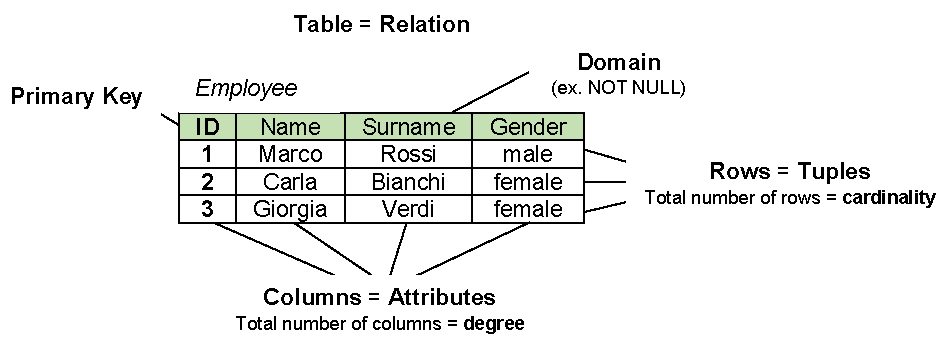
\includegraphics[scale=.75]{figures/relational_model.pdf}
\centering
\caption{Relational model concepts in a trivial example. `Employee' is the name of the real-world entity of reference and therefore of the related table in the model.}
\label{fig:relational_model}
\end{figure}

Lastly, since this term will be often used in the subsequent sections and chapters, we define a \textbf{dataset} as a collection of data. More specifically, since our data are in a tabular format according to the relational model, a dataset simply corresponds to one or more database tables.

Further details on relational databases can be found in \cite{abiteboul1995foundations}.


\section{Data Science Pipeline}
\label{section:data_science_pipeline}
Because of the broadness of the concept, there is not a unique and precise definition of data management. In general, we can identify it as the process of acquiring, storing, organizing, and maintaining data created and collected by an organization. In \cite{gandomi2015beyond}, the author, referring to \cite{labrinidis2012challenges}, classifies \textit{data management}, together with \textit{analytics}, as one of the two sub-processes to extract insights from data, while the overarching process is referred as \textbf{data science pipeline}, or \textit{big data pipeline}. For the sake of clarity, since the term is the one used in \cite{gandomi2015beyond}, we define big data as:
\begin{quote}\emph{Large volumes of high velocity, complex and variable data that require advanced techniques and technologies to enable the capture, storage, distribution, management, and analysis of the information.} \cite[p.~10]{mills2012demystifying}\end{quote}
However we preferred to adopt the name of `data science pipeline' instead of `big data pipeline', since we will not deal with big data, which are not a concept strictly inherent to this research.

\begin{figure}[t!]
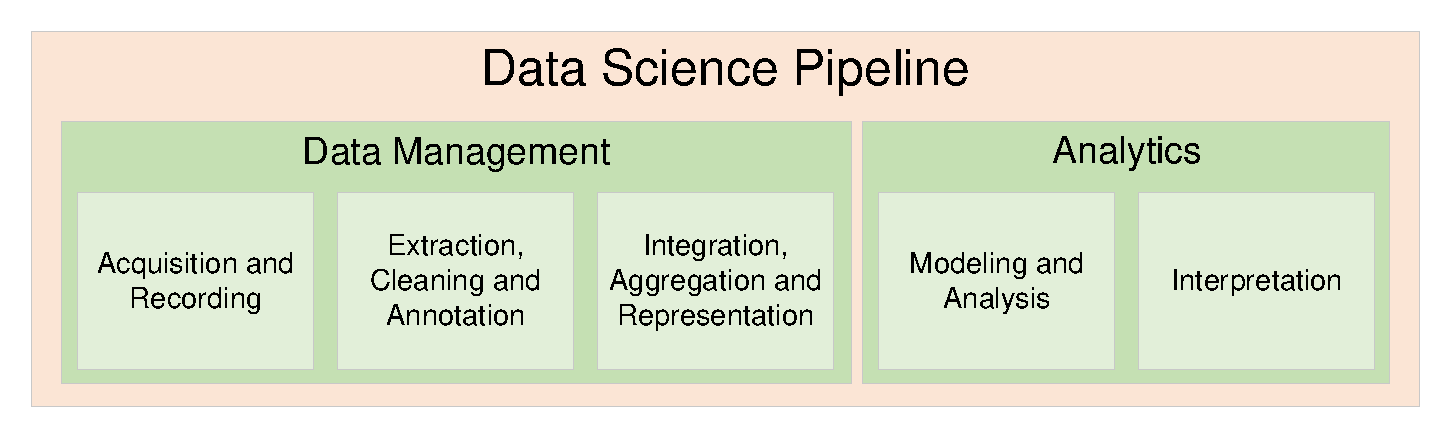
\includegraphics[scale=.5]{figures/data_science_pipeline.pdf}
\centering
\caption{Data science pipeline. Image based on the one shown in \cite{gandomi2015beyond}.}
\label{fig:data_science_pipeline}
\end{figure}

Since fairness should be addressed in each phase of the data science pipeline, the subsequent list provides a concise explanation of the operations performed in each step, by following the classification proposed in \cite{jagadish2014big}, together with the main potential sources of bias.
\begin{itemize}
\item \textbf{Acquisition and recording}: data are recovered and captured. In this phase the introduction of bias could derive from some preliminary critical choices we have to deal with, concerning the availability of sources, the identification of who is represented by the data, the definition of what has been measured and of our duties to the people in the data (for example, we may owe them a certain degree of privacy).
\item \textbf{Extraction, cleaning and annotation}: real data are most of the time messy and dirty, therefore we need to extract the relevant information and clean them, in order to express them in a structured form suitable for analysis. Unfortunately, data cleaning itself is based on assumptions, and wrong assumptions may lead to bias (for example, we may assume missing values in the data as missing at random, while there could be other, maybe ethical, reasons behind).
\item \textbf{Integration, aggregation and representation}: data analysis often requires the collection of heterogeneous data from different sources, therefore we need to integrate them in order to guarantee syntactic and semantic coherence. Again, we have to rely on assumptions on the world, as for the case of data representation, in which a lot of choices are made in order to decide what to represent, potentially leading to bias (for example, in the context of sentiment analysis we may ascribe sentiment to labels, or we may decide to group age values instead of considering every single year).
\item \textbf{Modeling and analysis}: before the actual analysis, an abstract model of the data is generated, in order to capture the essential components of the system and their interactions. However, the process of abstraction of concrete data in a conceptual standard model necessarily leads to the loss of information (for example, the relational model provides an intuitive overview of the system, but it does not include any semantics).
\item \textbf{Interpretation}: a decision-maker, provided with the results of the analysis, has to interpret these results. This process usually requires to examine all the assumptions made and to retrace the analysis, and because of the complexity of the task and the problems that may arise from computer systems (bugs, errors), a human (and therefore impossibly perfectly fair) supervision is needed (for example, the failures of system components can go unnoticed and result in loss of data, or the data format may have changed without being notified, and therefore the system should be equipped with monitoring scripts and mechanisms to obtain user confirmation and correction).
\end{itemize}


\section{Data Mining Techniques}
\label{section:data_mining_techniques}
\begin{quote}\emph{Data mining is a collection of techniques for efficient automated discovery of previously unknown, valid, novel, useful and understandable patterns in large databases.} \cite[p.~80]{tamilselvi2015efficient}\end{quote}
Data mining is a broad topic, and usually a variety of procedures are needed in order to gain knowledge from data. However, we can distinguish three main categories of techniques, in each of which the fairness problem should be addressed differently:
\begin{itemize}
\item \textbf{Preprocessing techniques}: procedures used to transform the raw data in a useful and efficient format. The aim is to improve the overall quality of the data and consequently the data mining results.
\item \textbf{Inprocessing techniques}: data are subjected to various methods using machine learning and artificial intelligence algorithms to generate a desirable output.
\item \textbf{Postprocessing techniques}: methods to evaluate the extracted knowledge, visualize it, or merely document it for the end user. The knowledge can also be interpreted and incorporated into an existing system.
\end{itemize}

For the purpose of this research, we will focus on preprocessing techniques, which constitute one of the most critical steps in the data mining process, since they deal with the preparation and transformation of the initial dataset; while the bias analysis we will perform making use of the tools adopted is part of data (in)processing. Data preprocessing methods are divided into four categories \cite{tamilselvi2015efficient}:
\begin{itemize}
\item \textbf{Data cleaning}: since real-world data are often incomplete, noisy, and inconsistent, some routines are needed in order to fill in missing values, smooth out the noise and correct the inconsistencies.
For what concerns \textit{missing values}, these procedures include the removal of the specific tuple, or the filling (manual or automatic) of the missing value by using, for example, a constant (e.g. `unknown'), the mean (for numerical attributes) or simply what is perceived to be the most probable value.
Noise instead can be seen as a random error or variance in a measured variable, and some smoothing techniques for \textit{noisy data} are:
\begin{itemize}
\item \textbf{Binning}: a data value is smoothed by looking at its `neighborhood', that is, the values around it.
\item \textbf{Regression}: data are fitted to a function, in order to be smoothed according to the function itself. A specific type of regression, useful for our analysis, is \textit{linear regression}, which will be further explored in Section~\ref{section:linear_regression}.
\item \textbf{Clustering}: similar data are organized into groups of values, called `clusters'. Values that fall outside the set of clusters may be considered as outliers.
\end{itemize}
\item \textbf{Data integration}: as mentioned in Section~\ref{section:data_science_pipeline}, data often come from different (possibly heterogeneous) sources, and therefore they need to be combined in order to obtain a coherent model and remove inconsistencies (such as redundancies between attributes, where some can be derived from others).
\item \textbf{Data transformation}: data are transformed or consolidated in appropriate forms suitable for the mining process. Some techniques used in this context are:
\begin{itemize}
\item \textbf{Normalization}: data values are scaled so as to fall within a specified range, such as (\(-\)1.0, 1.0 or 0.0, 1.0).
\item \textbf{Aggregation}: new attributes are constructed from the given set of attributes to help the mining process by summarizing or aggregating information (for example, daily sales data may be aggregated so as to compute annual total amounts).
\item \textbf{Generalization}: raw (or low-level) data are replaced by higher-level ones, by following a specific hierarchy (for example, the attribute \textit{city} can be generalized to \textit{country}).
\item \textbf{Discretization}: raw values of numeric attributes are replaced by interval levels or conceptual levels (for example, age values between 15 and 18 could be labeled as `adolescence').
\end{itemize}
\item \textbf{Data reduction}: in order to make mining more effective and get better analytical results, several techniques can be applied to obtain a reduced representation of the dataset that is much smaller in volume, yet closely maintains the integrity of the original data. These methods include, among the others, \textit{attribute subset selection}, in which attributes considered as not particularly relevant for the analysis are removed, and \textit{numerosity reduction}, where data are replaced by smaller data representations, such as parametric models.
\end{itemize}


\section{Linear Regression}
\label{section:linear_regression}
In order to fully understand how one of the adopted tools works (the one we refer to as `Glassdoor Method', described later in Section~\ref{section:the_glassdoor_method}), it is appropriate to have a closer look at \textbf{linear regression} \cite{glasserman2001linear}. As mentioned in Section~\ref{section:data_mining_techniques}, linear regression is a preprocessing technique used to smooth out noise or to find patterns within a dataset, which attempts to model the relationship between two or more variables by fitting data to a linear equation (represented, in the two-variable case, by a straight line in a Cartesian plane). The results from linear regression help in predicting an unknown value depending on the relationship with the predicting variables. For example, the height and weight of an individual generally are related: usually taller people tend to weigh more. We could use regression analysis to help predict the weight of a person, given their height.

We can distinguish between \textbf{simple linear regression}, in which a single input variable is used to model a linear relationship with the target variable (as for the example of height and weight), and \textbf{multiple linear regression}, where more predicting variables are used.

For simple linear regression, the reference equation is: \[y = \beta_0 + \beta_1x + \epsilon\]
Variable \(x\) is called \textit{explanatory} or \textit{independent variable}, while \(y\) is referred to as \textit{dependent variable}; \(\beta_1\) is the \textit{slope} of the line, also known as regression coefficient, and \(\beta_0\) is the \textit{intercept} (the value of \(y\) when \(x = 0\)), while \(\epsilon\) is the \textit{error} in the estimation of the regression coefficient, also known as residuals, which account for the variability in \(y\) that cannot be explained by the linear relation between \(x\) and \(y\).

For multiple linear regression, the formula is generalized in order to encapsulate also the other independent variables (\(x_1, \ldots, x_n\)) and the related slope coefficients (\(\beta_1, \ldots, \beta_n\)): \[y = \beta_0 + \beta_1x_1 + \ldots + \beta_nx_n + \epsilon\]

\begin{figure}[t!]
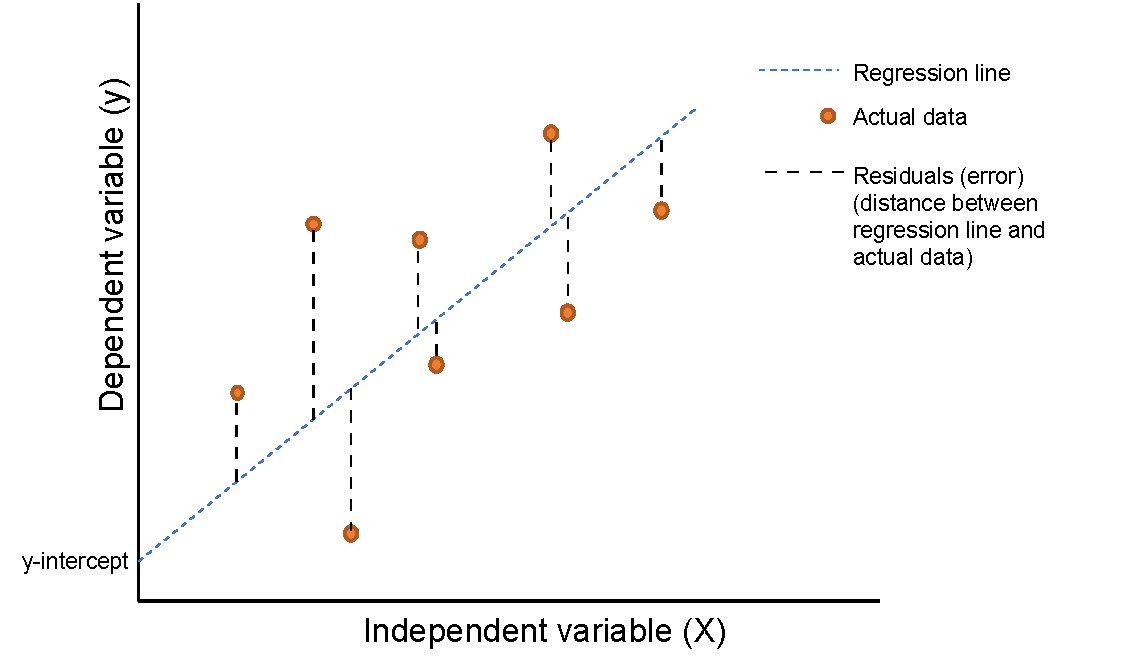
\includegraphics[scale=.7]{figures/simple_linear_regression.pdf}
\centering
\caption{Simple linear regression graph.\newline
Source: \upshape\protect\url{https://www.reneshbedre.com/assets/posts/reg/mlr/residual.svg}.}
\label{fig:simple_linear_regression}
\end{figure}

Figure~\ref{fig:simple_linear_regression} shows a simple linear regression graph. It is important to point out that the \(x\) and \(y\) variables remain the same, since they represent data features that cannot be changed, while the values that we can control are the slope and the intercept. Indeed, there can be multiple straight lines depending upon the values of intercept and slope, and what the linear regression algorithm does is to fit multiple lines on the data points and return the line that results in the least error.

Another important parameter for regression analysis is \(R^2\), also known as \textit{coefficient of determination} (or \textit{coefficient of multiple determination} for multiple linear regression). It is a statistical measure of how close the data are to the fitted regression line, and therefore it indicates how much variation of the dependent variable is explained by the independent variable(s) in a regression model. \(R^2\) values range from 0 to 1 and are commonly stated as percentages from 0\% to 100\%, where 0\% refers to a model that explains none of the variability of the data around its mean, while 100\% refers to a model that explains all the variability of the data around its mean (in this case, all the actual data values would be on the regression line).

Formally, we can define \(R^2\) as: \[R^2 = 1 - \frac{\mathit{Unexplained Variation}}{\mathit{Total Variation}} = 1 - \frac{\sum_{i}(y_i - \hat{y}_i)}{\sum_{i}(y_i - \bar{y})}\] where \(y_i\) is one of the actual data values, \(\hat{y}_i\) is the corresponding predicted value, and \(\bar{y}\) is the mean of all the \(y_i\) values, for \(i = 1, \ldots, n\).

Generally speaking, at least for the purpose of this research, the higher the \(R^2\) value, the better the model fits the data.


\section{Functional Dependencies}
\label{section:functional_dependencies}
One of the tools adopted, FAIR-DB, uses specific classes of integrity constraints, known as dependencies, to detect unfair behaviors in datasets (further details on the tool will be provided in Section~\ref{section:fair-db}). A \textbf{dependency} is a constraint that applies to or defines the relationship between attributes, and it occurs in a database when information stored in a table uniquely determines other information stored in the same table. Basically, dependencies are constraints not necessarily imposed by the system designer but intrinsically satisfied by the data.

\textbf{Functional Dependencies (FDs)} are a specific type of dependency, involving two (sets of) attributes of the same relation in which the first uniquely determines the second or, in other words, knowing the value of one attribute (or set of attributes) is enough to tell the value of the other one. The notation to indicate a functional dependency is: \[A \rightarrow B\] which can be read as `\(B\) is functionally dependent upon \(A\)', or `\(A\) uniquely determines \(B\)', whereas \(A\) and \(B\) are attributes (or eventually sets of attributes) of a table. \(A\) is called antecedent, or \textit{left-hand-side (LHS)}, and \(B\) consequent, or \textit{right-hand-side (RHS)}. An example of functional dependency could be the one of a table containing the information about the employees of a company, as in Figure~\ref{fig:relational_model}. Here the \(\mathit{ID}\) attribute uniquely identifies the \(\mathit{Name}\) one, because by knowing the employee's ID we can tell what the employee's name is. Therefore, \(\mathit{ID} \rightarrow \mathit{Name}\). More specifically, since also the employee's surname and gender are uniquely identified by the ID, we can write \(\mathit{ID} \rightarrow \mathit{Name}, \mathit{Surname}, \mathit{Gender}\). Another example is provided in Table~\ref{table:orange_plantation}, in which \(\mathit{Temperature}, \mathit{pH}, \mathit{Season} \rightarrow \mathit{Ideal}\).

\begin{table}[t!]
\begin{tabularx}{\columnwidth}{|Y|Y|Y|Y|}
\hline
\multicolumn{4}{|c|}{Orange Plantation}\\
\hline
Temperature & pH & Season & Ideal\\
\hline
28 & 7 & Autumn & Y\\
20 & 7 & Autumn & N\\
28 & 7 & Winter & N\\
29 & 7.5 & Autumn & Y\\
27 & 6.5 & Winter & N\\
27 & 7.5 & Summer & N\\
20 & 6.5 & Spring & N\\
28 & 7 & Summer & N\\
27 & 6.5 & Autumn & Y\\
\hline
\end{tabularx}
\centering
\caption{`Orange Plantation' table. It shows whether or not ambient temperature (\textdegree C), soil pH and planting season represent ideal conditions for planting oranges.}
\label{table:orange_plantation}
\end{table}

Functional dependencies are a very well-known concept for data scientists, especially for those who work on relational models, and further details on them can be found in \cite{abiteboul1995foundations}.
However, the constraints imposed by functional dependencies are often too strict for real-world datasets (they must indeed hold for all the tuples of a table), so in the past few years generalizations of FDs have been proposed and started to be considered in their place. \textbf{Relaxed Functional Dependencies (RFDs)} can indeed be simply defined as functional dependencies where some constraints are deleted (relaxed). The authors of \cite{caruccio2015relaxed} distinguished 35 different categories of RFDs, but the ones relevant for our research are the following:
\begin{itemize}
\item \textbf{Approximate Functional Dependencies (AFDs)}:
\begin{quote}\emph{AFDs are FDs holding on almost every tuple.} \cite[p.~151]{caruccio2015relaxed}\end{quote}
In order to quantify how an AFD `almost' holds, several measures have been proposed, including the so-called \textit{g3}, defined as ``the (normalized) minimum number of tuples that need to be removed from a relation instance in order for an FD to hold'' \cite[p.~151]{caruccio2015relaxed}, whereas `relation instance' is simply a synonym of `relation'. The g3 measure is therefore an index whose value ranges between 0 and 1, indicating the percentage of tuples of a table to be removed in order for an FD to hold (0 = none, 1 = all). An example of AFD in Table~\ref{table:orange_plantation} is: \[\mathit{Temperature}, \mathit{pH} \rightarrow \mathit{Ideal}\] because almost all the values of \(\mathit{Temperature}\) and \(\mathit{pH}\) determine the \(\mathit{Ideal}\) value, but this is not true for: \[\mathit{Temperature} = \mlq 28 \mrq, \mathit{pH} = \mlq 7 \mrq \rightarrow \mathit{Ideal}\] since in most of the cases (two out of three) when \(\mathit{Temperature} = \mlq 28 \mrq\) and \(\mathit{pH} = \mlq 7 \mrq\) then \(\mathit{Ideal} = \mlq \mathrm{Y} \mrq\), but in one case \(\mathit{Ideal} = \mlq \mathrm{N} \mrq\).
\item \textbf{Conditional Functional Dependencies (CFDs)}:
\begin{quote}\emph{\emph{[CFDs]} use conditions to specify the subset of tuples on which a dependency holds.} \cite[p.~152]{caruccio2015relaxed}\end{quote}
This type of dependencies allows to catch particular and concrete patterns in the dataset, in fact they make possible to analyze precise values of the tuples and be more specific. An example of CFD, related to Table~\ref{table:orange_plantation}, is the following: \[\mathit{Temperature} = \mlq 28 \mrq, \mathit{pH} = \mlq 7 \mrq, \mathit{Season} \rightarrow \mathit{Ideal}\] meaning that, for tuples in which \(\mathit{Temperature} = \mlq 28 \mrq\) and \(\mathit{pH} = \mlq 7 \mrq\), the \(\mathit{Season}\) parameter functionally determines the \(\mathit{Ideal}\) one. Another example could be: \[\mathit{Season} = \mlq \mathrm{Summer} \mrq \rightarrow \mathit{Ideal} = \mlq \mathrm{N} \mrq\] interpretable as: `when the attribute \(\mathit{Season}\) has value \(\mathrm{Summer}\), the attribute value of \(\mathit{Ideal}\) is \(\mathrm{N}\)'.
\item \textbf{Approximate Conditional Functional Dependencies (ACFDs)}: FDs obtained by combining the two kinds of relaxed dependencies discussed above. Unifying the two relaxation criteria makes it possible to detect specific and not exact rules, which can highlight anomalies or unexpected patterns in the database, allowing to recognize cases where a value of a certain attribute \textit{frequently determines} the value of another one. An example of ACFD in Table~\ref{table:orange_plantation} is: \[\mathit{Season} = \mlq \mathrm{Autumn} \mrq \rightarrow \mathit{Ideal} = \mlq \mathrm{Y} \mrq\] which can be read as: `when attribute \(\mathit{Season}\) has value \(\mathrm{Autumn}\), the attribute value of \(\mathit{Ideal}\) is \(\mathrm{Y}\) if we delete a maximum number of tuples \(N\) from the dataset'. The rule indeed holds for almost all the tuples of the table, apart for the one in which \(\mathit{Temperature} = \mlq 20 \mrq\), \(\mathit{pH} = \mlq 7 \mrq\), \(\mathit{Season} = \mlq \mathrm{Autumn} \mrq\) and \(\mathit{Ideal} = \mlq \mathrm{N} \mrq\). It is worth to specify that, even though the notation is the same used for CFDs, the relaxation on the number of tuples is implicit in the classification of a rule as an ACFD.
\end{itemize}


\section{Evaluation Metrics}
\label{section:evaluation_metrics}
The aim of this section is to introduce some evaluation metrics for functional dependencies used by one of the adopted tools, FAIR-DB, described later in Section~\ref{section:fair-db}.

\begin{itemize}
\item \textbf{Support}: \[\mathrm{Support}(X \rightarrow Y) = \mathrm{supp}(X, Y) = \frac{\#(X, Y)}{\mathit{\#tuples}}\] where \(\#(X, Y)\) is the amount of times the (sets of) attributes \(X\) and \(Y\) appear together in the dataset and \(\#tuples\) is the total amount of tuples in the table. The support represents the percentage of records in the dataset that verify the dependency \(X \rightarrow Y\), and it is therefore an index whose value ranges between 0 and 1.
\item \textbf{Confidence}: \[\mathrm{Confidence}(X \rightarrow Y) = \mathrm{conf}(X, Y) = \frac{\mathrm{supp}(X, Y)}{\mathrm{supp}(X)}\] where \(\mathrm{supp}(X)\) is the percentage of tuples in the dataset containing the (set of) attributes \(X\) (antecedent, or LHS, of the rule). The confidence shows how frequently the dependency \(X \rightarrow Y\) is verified, knowing that the antecedent \(X\) is verified, and it is therefore an index whose value ranges between 0 and 1. A confidence equal to 1 means that only the valid and exact rules (non-relaxed FDs) will be selected, while decreasing its value implies relaxing the constraint on the number of tuples to be considered. In this context, it can be seen as an analogous metric to the g3 one, mentioned in Section~\ref{section:functional_dependencies}.
\item \textbf{Difference}: \[\mathrm{Difference}(X \rightarrow Y) = \mathrm{diff}(X, Y) = \mathrm{conf}(X, Y) - \mathrm{conf}(X \setminus X_p, Y)\] where \(X_p\) is the subset of protected attributes of the antecedent \(X\) of the dependency \(X \rightarrow Y\). The difference is basically a subtraction between the confidence value of a dependency and the confidence value calculated on the same dependency but excluding all the protected attributes from the antecedent of the rule. Being a subtraction of indexes of value between 0 and 1, and given \(\mathrm{conf}(X, Y) \geq \mathrm{conf}(X \setminus X_p, Y)\), the difference is also an index whose value ranges between 0 and 1. It indicates how much a dependency is `unethical' (the higher the value, the more unfair is the dependency), and it gives an idea on the impact of the protected attributes on \(Y\). Last but not least, it is important to point out that the difference is a novel metric, firstly introduced in \cite{azzalini2021fair} and specifically designed with the aim of measuring the `ethical' level of a dependency.
\end{itemize}


\section{Statistical Concepts}
\label{section:statistical_concepts}
The aim of this section is to introduce some statistical concepts useful for fully understanding the behavior of one of the adopted tools, Ranking Facts, described later in Section~\ref{section:ranking_facts}.

The first required notion is the one of a \textbf{hypothesis test}, which in statistics is a way to test the obtained result of a survey or experiment on a sample, in order to check if the result is meaningful and extendable to the whole population or if it has happened by chance. In this context, two interpretations are proposed: the first is known as \textit{null hypothesis} (symbolized as \(H_0\)), which is the idea that there is no relationship in the population and that the relationship in the sample is caused by errors (informally, this is the `occurred by chance' interpretation); the second is called \textit{alternative hypothesis} (whose symbol is \(H_1\)) and it is the idea that the relationship in the sample reflects an existing relationship in the population.

Generally, the rationale behind a hypothesis test is:
\begin{itemize}
\item[1.] Assume the null hypothesis true.
\item[2.] Determine how likely the sample relationship would be if the null hypothesis were true.
\item[3.] If the sample relationship would be extremely unlikely, then \textit{reject} the null hypothesis in favor of the alternative hypothesis. If it would not be extremely unlikely, then \textit{retain} the null hypothesis.
\end{itemize}

A crucial step in hypothesis testing is to find the likelihood of the sample result if the null hypothesis were true. This probability is called \textbf{\(\bm{p}\)-value}. Low \(p\)-value means that the sample result would be unlikely if \(H_0\) were true and leads to the rejection of the null hypothesis, while high \(p\)-value means that the sample result would be likely if \(H_0\) were true and leads to the retention of the null hypothesis. To quantify how low the \(p\)-value must be in order to consider the result unlikely enough to reject the null hypothesis, a parameter known as \textit{significance level} \(\alpha\) is used, and its value is usually set to 0.05 (5\%). The significance level represents the probability of making the mistake of rejecting the null hypothesis when in fact it is true (\textit{type I error}): if \(p\textrm{-value} > \alpha\) we accept the null hypothesis and the result is considered not statistically significant, otherwise we reject the null hypothesis and the result is said to be \textit{statistically significant}.

A particular type of hypothesis test is the \textbf{z-test}, used when data are approximately normally distributed (i.e. the plotted data have the shape of a bell curve on the graph). In order for a z-test to be used, data points should also be independent of each other and the sample size should be greater than 30. The z-test relevant to our research is the \textit{two sample z-test}, which allows to compare two proportions to check if they are the same (\(H_0\)) or not (\(H_1\)). The reference formula is: \[z = \frac{p_1 - p_2}{\sqrt{(\frac{\sigma_1^2}{n_1} + \frac{\sigma_2^2}{n_2})}} = \frac{p_1 - p_2}{\sqrt{p(1 - p)(\frac{1}{n_1} + \frac{1}{n_2})}}\] where \(n_1\) and \(n_2\) are the sizes of the samples, \(p_1\) and \(p_2\) are the proportions of the samples, \(p\) is the overall sample proportion (total number of `positive' results over total number of people) and \(\sigma_1^2\) and \(\sigma_2^2\) represent the variances of the two populations. For the sake of completeness, we define the \textit{variance} as the measure of how far each value in the dataset is from the average value (i.e. the mean, as defined in Section~\ref{section:the_glassdoor_method}): \[\sigma^2 = \frac{\sum\limits_{i=1}^n (x_i - \mu)^2}{n}\] where \(n\) is the size of the population, \(x_i\) is the \(i\)-th value and \(\mu\) represents the mean. In the z-score formula above, for the sake of simplicity, \(\sigma_1^2\) and \(\sigma_2^2\) are approximated by the variance of the Bernoulli distribution (i.e. the probability distribution for a random experiment with only two possible outcomes). To better clarify, we will now consider the example of testing two different COVID-19 vaccines: the first works on 248 people out of a sample of 496, while the second works on 23 people in a sample of 100. To check if the vaccines are comparable we firstly calculate the proportions: \[p_1 = 248 / 496 = 0.5\] \[p_2 = 23 / 100 = 0.23\]
The overall sample proportion is: \[p = \frac{248 + 23}{496 + 100} \simeq 0.45\]
And finally the z-score is: \[z \simeq \frac{0.5 - 0.23}{\sqrt{0.45(1 - 0.45)(\frac{1}{496} + \frac{1}{100})}} \simeq 4.95\]
To find out if the obtained result should lead us to accept or reject the null hypothesis, we can look at the known values of z-score, related to the most commonly used \(\alpha\) values. For example, the z-score related to \(\alpha = 0.05\) is 1.96, meaning that 95\% of the area under the normal curve lies within the range \([-1.96, +1,96]\), and since \(4.95 > 1.96\) we can reject the null hypothesis (for z-scores higher than 1.96 with \(\alpha = 0.05\), \(p\textrm{-value} < 0.05\)).
